\documentclass{article}
\usepackage{amsmath, amsfonts, amsthm, amssymb}  
\usepackage{secdot}
\usepackage{epsfig}
\usepackage{fancyvrb}
\usepackage{cprotect}
\usepackage[T1]{fontenc}
\usepackage{epstopdf}
\usepackage{url}
\usepackage{rotating}
\usepackage{graphicx}
\usepackage{caption}
\usepackage{subcaption}
\usepackage{multirow}
\usepackage{setspace}
\usepackage{array}
\usepackage{fancyhdr}
\usepackage{lastpage}
\usepackage[T1]{fontenc}

\usepackage{geometry}
\geometry{letterpaper, left=1in, right=1in, top=1in, bottom=1in}

\pagestyle{fancy}
\fancyhf{}
\rhead{\thepage/\pageref{LastPage}}
\lhead{OSU ECEN 2233 - Logic Design - Fall 2024}
\rfoot{\LaTeX}


% ----- Identifying Information -----------------------------------------------
\newcommand{\myassignment}{Project: Increasing Throughput with SHA}
\newcommand{\myduedate}{Assigned: Monday 10/28; Due \textbf{Friday 12/6} (midnight)}
\newcommand{\myinstructor}{Instructor: James E. Stine, Jr.}
% -----------------------------------------------------------------------------

\begin{document}
\begin{center}
  {\huge \myassignment} \\
  {\large \myduedate} \\
  \begin{flushright}
  \myinstructor \\
  \end{flushright}
\end{center}

\section{Introduction}

This project is meant to be an encompassing project that gives you the
full experience of all that you learned in this course.  It will bring
ideas that we covered as well as had within laboratories.  It will
also try to reinforce all the skills you learned during your time in
laboratory.

This project is significantly involved compared to our normal labs
and much of the detail is left
up to you to implement.  Unfortunately, we cannot monitor your
process, therefore, it is important to allocate your
time wisely and come into laboratory every week.  Do not assume you
can do much of the work later or will have time to make up time later.
To make things worse, we only have one
week when we return from Thanksgiving making it almost impossible to
complete the project during that final week.  That is, you should
complete most of the project items before Fall Break and the
Thanksgiving Holiday.  Waiting until the final week will be a guaranteed
disaster for you.  

When designing digital systems, the process of creating logic to
accomplish some form of computation is a function of the blocks that
can be utilized.  Many times, the only way to increase the amount of
computation is to process more and more data in parallel.  However,
sometimes computation needs to be processed independently per block
and the only way to increase the computation time is to increase the
amount that can happen per time.  This is sometimes called
throughput.


\section{Background}

Throughput can be visualized with a kitchen.  Suppose that someone only
has $1$ oven in their kitchen.  Obviously, the cook is limited by the
amount of time that can complete a dinner by how often I can use this
oven.  On the other hand, if I am fortunate to have $2$ ovens in my
kitchen, I can use this to help do more things at the same time.  This
processing power is predicated on the fact that each oven probably is
not used at the same time and some foods cook faster than others.
Therefore, sequencing the oven to use it optimally is the key to
making throughput work effectively.

In digital systems, one way we can increase the throughput for a
design is to add a register where one stores intermediate results.
These intermediate results are typically stored into a group of flip
flops or a register and fed back into the register to get to the final
computation.  The use of registers helps optimize this throughput and
also increases the latency of the computation by increasing the clock
rate.

For example, suppose a computation needs to pass through $4$
adders to form the final result and stored into a register.
Also, assume that each adder
completes its operation in $100$ ns and stores the result into a
register.  In theory, this would be $4 \times 100 = 400$~ns to
complete the operation.
If a designer removed $3$ of these adders and
added a register following an adder (note: the result would need to go back
into the adder $3$ more times to complete the operation as shown in
Figure~\ref{throughput1.fig}).
For both of these scenarios, it
would still take a little time to store/read the value from a
register, but for this example, I am assuming that this amount is
negligible.  
However, the first unit can only be clocked at $1/400ns = 2.5$ MHz,
however, the second version could be computed at $1/100ns = 10.0$ MHz and run
significantly faster.  If a company is designing this hardware to process $100,000$
operations, the first version can only process all of these items in
$40$ msec, whereas, the clocked version takes $10$ msec.  This is a
$4$x speedup and significant improvement in latency for the total
operation.
Most importantly, the second architecture may have less area
than the first architecture.  Typically, more registers can increase energy
consumption, however, if you can significantly gain performance by increasing
throughput with a small increase in energy, it is often worth the
investment.  This is what we are investigating for this project or
increasing the throughput of our design.
\begin{figure} [t!]
  \centering
  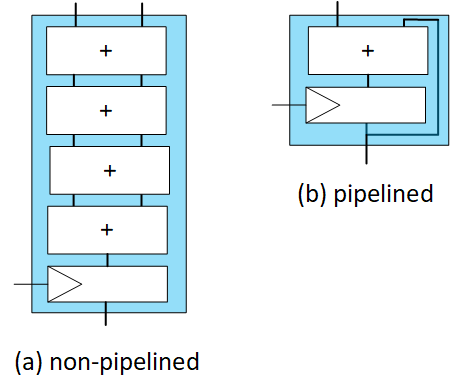
\includegraphics[scale=1.2]{throughput1.png}
  \caption{Adding registers to increase throughput}
  \label{throughput1.fig}
\end{figure}

The key to digital systems is that digital logic can process data in
parallel.  This project involves taking Laboratory $2$ and modifying
it to include a register to increase throughput and performance.
In order to complete this project, the following items must be
functional on the board:
\begin{itemize}
\item Control logic should be added to control each iteration of the
  unit to compute the SHA-256 operation.
\item All testbenches for the system, control, and datapath.
\item Use of the ILA to test your design (see Section~\ref{ila.sec})
\item Cleaned up code removing any unnecessary logic and/or states.
\item A report documenting the complete system and its operation
  indicating that it is working.
\item Anything you can think of to promote your project!
\end{itemize}

This project is not difficult and it is an excellent
choice for groups that want a straightforward
project and/or who wish to spend a minimal amount of time as possible on the project. However,
it is in your best interest to make the project better! Any modification beyond the baseline
project will incur extra points that could help compensate for a bad test, missing homework, or
bad quiz. The following are potential modifications you can easily add
for extra credit:
\begin{itemize}
\item Add more operations (e.g., SHA-512)
\item Add some way to add a new input message to the unit as opposed
  to hard coding the messages.
\item Determine a way to optimize the operation of the register to
  process throughput faster (e.g., adding another \verb!main_comp!
  block so that it completes faster and balances the timing between clocking)
\item Determine the best timing to optimize the throughput
\item Add a poster to explain to the masses!
\item Create a YouTube\textsuperscript{\textcircled{R}} channel on this project.
\end{itemize}

\section{Implementation}
\label{implementation.sec}

The basic idea for the inputs and output includes your move which you
should add through the switches.  You will technically only need a
``Start'' signal to get things going in the FSM.  As explained in
class, you should create the FSM intelligently, so that it can
theoretically process more data when needed.

The main key elements of the design will be provided to you, such as
the \verb!sha256.sv! module.  But, you will have to add registers,
control logic (e.g., Finite State Machines), multiplexors, input/output signals.
It is advisable to use as many input/output signals to help you debug
what is going on as you simulate and get to your final
implementation.

You should use many of the elements discussed in our
textbook~\cite{ddca-riscv}.  I would highly advise using the
\textit{idioms} we discussed in class 
and in the textbook for things
like registers making sure that you also reset or enable them appropriately.
That is, you should also incorporate a \textbf{reset} somewhere into your
design.  All of the HDL discussed in the textbook~\cite{ddca-riscv} is
on Canvas as a zip file.  Some of the registers are also available in
the \verb!SV! subdirectory of your project repository.
Feel free to use this HDL in any way you wish.

Again, using sequential logic to increase the throughput of a system involves
adding stages of registers or pipelines to split complex tasks into
smaller, manageable steps that can be processed concurrently. This
approach improves throughput by allowing different stages of a task to
be processed simultaneously, leading to an overall increase in the
number of tasks completed per unit time.

As explained previously there are many advantages in this process, but
there are also disadvantages.  As explained in class, the key to any
engineering system is making sure that you have more advantages than
disadvantages for it to be successful.  Some advantages to this
approach are: increased throughput, reduced latency per task, enhanced
resource utilization, and scalability.  The disadvantage to this
process is that its more challenging and complex than a traditional
serial approach.  There are other disadvantages, such as minimal
increase in latency, but for the most part using this approach saves a
ton of time.  That is, carefully balancing these trade-offs is key to
effectively using sequential logic to optimize throughput.

To make sure your implementation works, you should use some kind of an
enabled flip
flop (i.e., \verb!flopenr.sv!) that stores data when needed.
The FSM will be utilized to make sure these registers are written at
the right time.  You can utilize the methodology in class to design
the datapath and control of this design, however, any approach that is
reasonable also works.

\subsection{Integrated Logic Analyzer (ILA)}
\label{ila.sec}

In Lab~$2$, we used the $7$-segment display to display the final
result.  Although this works, many designers use Field Programmable
Gate Array (FPGA) features for debugging called the Integrated Logic
Analyzer (ILA).  In the 1970s and 1980s, many logic designers utilized
separate units that enabled them to debug items going on in their
logic.  These Logic Analyzers, such as the Tektronix LV-500, enabled
designs to be tested somewhat automatically.  However, with the advent
of the FPGA, these ideas could be automatically integrated into the
FPGA logic. More importantly, with this idea and a little ingenuity,
you can theoretically monitor internal signals.

For this laboratory, we are going to use the ILA from AMD.
The customizable Integrated Logic Analyzer (ILA) IP core is a logic
analyzer core that can be used to monitor the signals of a
design. The ILA core includes many advanced features of modern logic
analyzers, including Boolean trigger equations, and edge transition
triggers. Because the ILA core is synchronous to the design being
monitored, all design clock constraints that are applied to your
design are also applied to the components inside the ILA core.

These ILAs are not perfect in that they consume onboard memory blocks
that the FPGAs have.  So, in theory, you cannot probe all the signals
in your design.  However, not all signals usually need to be probed
using an ILA.
There is more information in the UG936 AMD (v2024.1) manual in the
docs directory.  We tried to put together a document in the
\verb!debug_tutorial! subdirectory of your repository.

You should decide which signals you would like to see if your design
is working.  Again,  you have the ability to probe a fair number of
signals in your FPGA, but be careful not to probe al your signals.
You can use the clock of the FPGA as the main driver for this ILA
block as documented in our debug document.

\section{Tasks}

Most of the main modules have been given to you to help you understand the
problem better.   In fact, we have given much of the project for you
in this text.  The difference here is that we have not given you an
testbenches and you will have to figure out how things go together.
You have all the skills you need to complete this project, so trusting
yourself and the process is worthwhile and I know all of you can do
this.  The tasks of the project are as follows:
\begin{enumerate}
  \item Add registers and any other logic to pipeline your system
    accordingly from \verb!sha256.sv!.  It is easiest to use $1$
    version of the \verb!main_comp! block and put registers after this
    unit.  You are welcome to determine the most optimal number of
    \verb!main_comp! blocks to use, but to get the baseline project
    done, I would use only $1$ block.
  \item Complete block diagrams of your system, include detailed
    interface specifications listing all signals and describing their
    timing.
  \item Design a control logic presumably with a FSM to have it work
  correctly.  Remember, the tip in Lab~$3$ to have the current state and next
  state output on your wave view to help debug things.
\item  Build the testbench to simulate your design and make sure
  things are working for both the datapath, control and combined
  datapath/control. It is advisable to make the datapath work first by
  creating a testbench that makes your datapath run.  Then, add the
  control logic to make sure your datapath works as needed.
  \item Once your design completely works, implement the design on
    the DSDB board.  You can still use the switches, push
    buttons, LEDs and also use the
    seven segment display to output key elements of your project.
    Remember, to use the LEDs to help you debug your design.
  \item Document the output of ILA for the message and hashed output.
    You can use the ILA to debug your design, as well.  This should be
    significantly easier than using other items (e.g., $7$-segment
    display).  Once you have the ILA set up, it is conceivably easy to
    run over and over.
  \item Finally compare the PPA of both designs and provide a
    justification if this project's design can process $1$ million SHA
    vectors faster or slower than Lab~$2$'s implementation.  Please be
    aware that the area of your ILA-enabled design my be larger due to
    the added items needed to support the ILA.  The resource output
    should actually document the ILA's PPA separately.  
\end{enumerate}

Again, the process here is not difficult.  If you need to work out any
of the procedures or ask me to inspect your design, I would recommend
stopping by to ask questions or advice.  I would not advise waiting
until the last week to start as I might be busy with
end-of-the-semester duties and starting early is the best practice.

The easiest way to make sure your control logic stops iterating
correctly is to use a counter.  There is a $64$-count counter in the
\verb!SV! subdirectory of your repository.  This is just a helpful
file that can give you a pathway towards a solution.  You are welcome
to use any pathway you wish to finalize your design.  There are some
other files in this subdirectory as well, such as registers and
multiplexors that will help you too. 

\subsection{Extra Credit}

There are lots of opportunities for extra credit with this project.
But, please, first focus on completing the baseline project before
attempting the extra credit option.  One of the advantages of digital
logic is that many bits can be computed in parallel and then chosen
later to be correct or incorrect.

Because Field Programmable Gate Arrays
(FPGAs) can contain many millions of logic gates, you can do lots of
optimization for this project.  Timing is challenging in this lab and
making sure your design works for multiple messages requires some
thought in how to process things accordingly.

\section{Video and Lab Report}

I am asking for
both a final report and video demo of your design.  You can easily
create a video on your cell phone that is no more than $5$-$10$ minutes
that encapsulates your design and how it works.  Please work
consistently throughout the final weeks of the semester to make sure
you complete the project on time.

I will also give extra credit to those that put a little effort into
making an outstanding video and showcasing their project in detail.
You could also potentially discuss other topics including significant
additions to your project.

You are also required to submit a final report of your design using
the lab rubric.  You should remember to submit both your lab report
and video report to Canvas for
your team, but please also submit your team evaluation, as well.
Beware; no
late projects will be accepted and if you miss submitting your project
on time, you will receive a $0$ for your project grade!  This
procedure should be similar to what you are using for your labs.
You should also take a printout of your waveform 
from your ModelSim simulation.  
Only one of your team members should upload
the files, lab report, and team assessment.  Also, please make sure you
hand in all files, including your HDL, testbenches, and other
important files you wish for us to see.

For the final project, you cannot use ``oops'' days to help you.  The
project is due December 6, 2024 at midnight.  If you are running late,
please hand in something.  If you decide not to hand in anything, you
will receive a $0$ for the project.   Only medical or family
emergencies that are clearly documented for getting any extensions.
Even if you get an extension, it will be difficult as the University
closes the Endeavor building early.  Also, please be aware that
Thanksgiving week falls at a bad time this year. Typically, you have
two weeks after Thanskgiving before the semester ends.  Unfortunately,
this year only has one additional week and you will probably not get
anything done then.  I highly recommend trying to get as much done
before the Thanksgiving break to avoid any issues.  

Please contact James Stine (james.stine@okstate.edu) 
for more help.  Your code should be
readable and well-documented. In addition, please turn in additional
test cases or any other added item that you used. 
Please also remember to document everything in your Lab Report using
the information found in the Grading Rubric.

   
\bibliographystyle{IEEEbib}
\bibliography{project}

\end{document}
